%\documentclass[aspectratio=169]{beamer}
\documentclass[10pt,aspectratio=169,xcolor={table,dvipsnames,usenames}]{beamer}
\usefonttheme[onlymath]{serif}
\usepackage[brazilian]{babel}


\mode<presentation>
{
  \usetheme{Madrid}      % or try Darmstadt, Madrid, Warsaw, ...
  \usecolortheme{dolphin} % or try albatross, beaver, crane, ...
  \usefonttheme{default}  % or try serif, structurebold, ...
  \setbeamertemplate{navigation symbols}{}
  \setbeamertemplate{caption}[numbered]
  \setbeamertemplate{headline}{}
}

\usepackage{mathtools}
%\usepackage{amsthm}
\usepackage{amsmath}
%\usepackage{nccmath}
\usepackage{amssymb}
%\usepackage{amsfonts}
\usepackage{physics}
%\usepackage{dsfont}
%\usepackage{mathrsfs}
%\usepackage{slashed}    % Feynman slash notation, requires LuaLaTeX
%\usepackage[compat=1.1.0]{tikz-feynman}   % Feynman diagrams

%\usepackage{titling}
\usepackage{indentfirst}
%\usepackage[titletoc,title]{appendix}
%\renewcommand\appendixname{Apêndice}

\usepackage{bm}
%\usepackage{xcolor}
%\usepackage[dvipsnames]{xcolor}
\usepackage{cancel}

%\usepackage{xurl}
\usepackage{hyperref}
\usepackage{cite}

\usepackage{float}
\usepackage{graphicx}
\usepackage{tikz}
\usepackage{caption}
\usepackage{subcaption}

%%%%%%%%%%%%%%%%%%%%%%%%%%%%%%%%%%%%%%%%%%%%%%%%%%%

\newcommand{\eps}{\epsilon}
\newcommand{\vphi}{\varphi}
\newcommand{\cte}{\text{cte}}

\newcommand{\N}{\mathbb{N}}
\newcommand{\Z}{\mathbb{Z}}
\newcommand{\Q}{\mathbb{Q}}
\newcommand{\R}{\vb{R}}
\newcommand{\C}{\mathbb{C}}
\renewcommand{\S}{\vb{S}}
%\renewcommand{\H}{\s{H}}

\renewcommand{\a}{\vb{a}}
\renewcommand{\b}{\vb{b}}
\renewcommand{\d}{\dagger}
\newcommand{\up}{\uparrow}
\newcommand{\down}{\downarrow}
\newcommand{\hc}{\text{h.c.}}

\newcommand{\0}{\vb{0}}
\newcommand{\1}{\mathds{1}}
\newcommand{\E}{\vb{E}}
\newcommand{\B}{\vb{B}}
\renewcommand{\v}{\vb{v}}
\renewcommand{\r}{\vb{r}}
\renewcommand{\k}{\vb{k}}
\newcommand{\p}{\vb{p}}
\newcommand{\q}{\vb{q}}
\newcommand{\F}{\vb{F}}
\newcommand{\A}{\vb{A}}
\newcommand{\J}{\vb{J}}

\newcommand{\s}{\sigma}
\newcommand{\nn}[2]{\left\langle #1 , #2 \right\rangle}
\newcommand{\cc}[1]{\overline{#1}}
\newcommand{\Eval}[3]{\eval{\left( #1 \right)}_{#2}^{#3}}

\newcommand{\unit}[1]{\; \mathrm{#1}}

\newcommand{\n}{\medskip}
\newcommand{\e}{\quad \mathrm{e} \quad}
\newcommand{\ou}{\quad \mathrm{ou} \quad}
\newcommand{\virg}{\, , \;}
\newcommand{\ptodo}{\forall \,}
\renewcommand{\implies}{\; \Rightarrow \;}
%\newcommand{\eqname}[1]{\tag*{#1}} % Tag equation with name


%%%%%%%%%%%%%%%%%%%%%%%%%%%%%%%%%%%%%%%%%%%%%%%%%%%%%%%%%

\title[Introdução ao Twisted Bilayer Graphene]{\LARGE{Introdução ao Twisted Bilayer Graphene}}
\author[Mateus Marques]{
\large{Mateus Marques
}}
\date{\today}

\begin{document}

\begin{frame}
  \titlepage
\end{frame}


\begin{frame}%{Grafeno}

\begin{itemize}
\item O grafeno é derivado do grafite (do seu lápis)

\item Uma única camada de grafite e mantido estável num substrato (SiO$_2$, hBN etc.)

\item Cristal 2D de átomos de carbono numa rede hexagonal (favo de mel)

\item Pelas ligações covalentes C$-$C, é cerca de 200 vezes mais forte que o aço

\item Incrivelmente leve, flexível e quase completamente transparente

\item Conduz eletricidade melhor do que o cobre, dissipa calor de maneira extremamente eficiente
\end{itemize}

\begin{figure}[H]
\centering
\includegraphics[height=0.25\linewidth]{fig/graphene.png}
%\caption{Estrutura do grafeno. Figura retirada de \url{https://sitn.hms.harvard.edu/flash/2011/graphene-the-coolest-material-that-shouldnt-exist/}.}
\label{fig:graphene}
\end{figure}

\end{frame}

%%%%%%%%%%%%%%%%%%%%%%%%%%%%%%%%%%%%%%%%%%%%%%%%%%%%%%%%%%%%%%%%%%%%%%%%%%%%%%%%%%%%%%%%%%%%%%%%%

\begin{frame}%{Padrão de moiré}

Quando empilhamos apenas duas camadas de grafeno, e giramos elas por um ângulo $\theta$, forma-se um padrão de interferência (de moiré).

\begin{figure}[H]
\centering
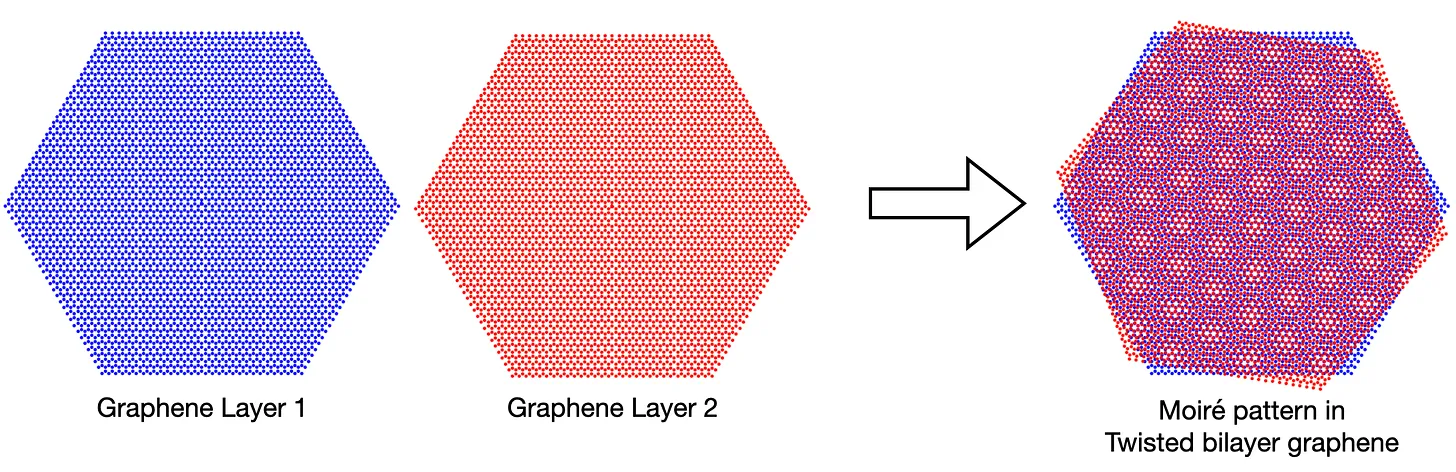
\includegraphics[height=0.32\linewidth]{fig/moire.png}
%\caption{Padrão de moiré. Figura retirada de \url{https://arpitarora22.substack.com/p/artful-probe-for-quantum-magic-in}.}
\label{fig:moire}
\end{figure}

\end{frame}

%%%%%%%%%%%%%%%%%%%%%%%%%%%%%%%%%%%%%%%%%%%%%%%%%%%%%%%%%%%%%%%%%%%%%%%%%%%%%%%%%%%%%%%%%%%%%%%%%

\begin{frame}%{Super periodicidade}

Para pequenos ângulos de torção, o padrão moiré produzido pela desorientação da rede entre as camadas bidimensionais de grafeno cria uma modulação de longo alcance da ordem de empilhamento. Temos uma matriz efetivamente periódica de regiões de empilhamento AA, formando uma rede hexagonal, e regiões de empilhamento AB e BA, formando uma rede em favo de mel, cuja periodicidade representa a nova escala de periodicidade do sistema.

\begin{figure}[H]
\centering
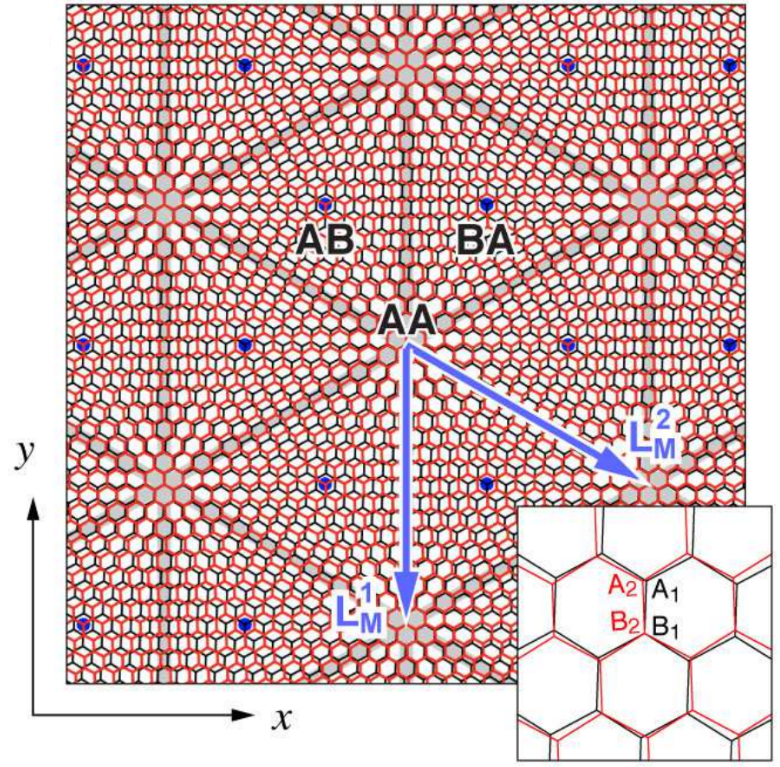
\includegraphics[height=0.32\linewidth]{fig/AA_AB.png}
%\caption{Padrão de moiré. Figura retirada de \url{https://arpitarora22.substack.com/p/artful-probe-for-quantum-magic-in}.}
\label{fig:AA_AB}
\end{figure}


O número de átomos de carbono na célula unitária da estrutura periódica gerada aumenta com a diminuição do ângulo de torção; para $\theta=1.1^\circ$, há aproximadamente 11000 átomos [6]. Quando o ângulo de torção do grafeno bicamada torcido (TBG) está próximo do ``ângulo mágico'' teoricamente previsto, a hibridização entre camadas induz quatro quase bandas planas de baixa energia. Estas exibem estados isolantes em meio preenchimento, que não são esperados na ausência de correlações entre elétrons, o que pode ser.

\end{frame}


%%%%%%%%%%%%%%%%%%%%%%%%%%%%%%%%%%%%%%%%%%%%%%%%%%%%%%%%%%%%%%%%%%%%%%%%%%%%%%%%%%%%%%%%%%%%%%%%%

\begin{frame}{Objetivos}

\begin{itemize}
\item Passar uma ideia introdutória de como generalizar a teoria BCS para estudar a \textbf{fenomenologia} da supercondutividade não-convencional.

\n\n

\item A inclusão de interações repulsivas e magnéticas causam anisotropia na função de gap.

\n\n

\item Entender a distinção básica das diferentes simetrias (jargão) s, p, d, f-wave.

\n\n

\item Existem mecanismos além dos fônons que geram interações atrativas?

\n\n

\item Foco específico nos cupratos e na simetria d-wave.
\end{itemize}

\end{frame}


%%%%%%%%%%%%%%%%%%%%%%%%%%%%%%%%%%%%%%%%%%%%%%%%%%%%%%%%%%%%%%%%%%%%%%%%%%%%%%%%

\begin{frame}{Referências}

\footnotesize

\begin{thebibliography}{10}
\bibitem{coleman}
\alert{P. Coleman.}
\newblock {Introduction to Many-Body Physics.}
\newblock {Cambridge University Press, 2015.}

\bibitem{timm}
\alert{Carsten Timm.}
\newblock {Theory of Superconductivity.}
\newblock {Version: March 24, 2023.}

\bibitem{tsuei}
\alert{C. C. Tsuei and J. R. Kirtley}
\newblock {Pairing symmetry in cuprate superconductors.}
\newblock {\textit{Rev. Mod. Phys.}, 72, 969, October 2000.}

\bibitem{wiki-cuprate}
\alert{Wikipédia contributors.}
\newblock {Cuprate superconductor - Wikipédia}
\newblock {\url{https://en.wikipedia.org/wiki/Cuprate_superconductor}.}

\end{thebibliography}


\end{frame}

\end{document}
